\chapter{Nuclear solutions}
\begin{abox}
	Practice Set 1 
	\end{abox}
\begin{enumerate}
	\item  The radius of a ${ }_{29}^{64} \mathrm{C} u$ nucleus is measured to be $4.8 \times 10^{-13} \mathrm{~cm}$.\\
	\textbf{(A)} The radius of $a{ }_{12}^{27} M g$ nucleus can be estimated to be
{	\exyear{NET/JRF(JUNE-2011)}}
\begin{tasks}(2)
\task[\textbf{A.}] $2.86 \times 10^{-13} \mathrm{~cm}$
\task[\textbf{B.}] $5.2 \times 10^{-13} \mathrm{~cm}$
\task[\textbf{C.}] $3.6 \times 10^{-13} \mathrm{~cm}$
\task[\textbf{D.}] $8.6 \times 10^{-13} \mathrm{~cm}$
\end{tasks}
\begin{answer}
\begin{align*}
\text{	Since }R&=R_{0}(A)^{1 / 3} \Rightarrow \frac{R_{M g}}{R_{C u}}=\left(\frac{A_{M g}}{A_{C u}}\right)^{1 / 3}=\left( \frac{27}{64}\right) ^\frac{1}{3}\\
\Rightarrow \frac{R_{M g}}{R_{C u}}&=\frac{3}{4} \Rightarrow R_{M g}=\frac{3}{4} \times 4.8 \times 10^{-13}=3.6 \times 10^{-13} \mathrm{~cm}
\end{align*}
So the correct answer is \textbf{Option (C)}
\end{answer}
\textbf{(B)} The root-mean-square (r.m.s) energy of a nucleon in a nucleus of atomic number $A$ in its ground state varies as:
\begin{tasks}(4)
\task[\textbf{A.}] $A^{4 / 3}$
\task[\textbf{B.}] $A^{1 / 3}$
\task[\textbf{C.}] $A^{-1 / 3}$
\task[\textbf{D.}] $A^{-2 / 3}$
\end{tasks}
\begin{answer}
So the correct answer is \textbf{Option (C)}
\end{answer}
\item The difference in the Coulomb energy between the mirror nuclei ${ }_{24}^{49} \mathrm{Cr}$ and ${ }_{25}^{49} \mathrm{Mn}$ is $6.0 \mathrm{MeV}$. Assuming that the nuclei have a spherically symmetric charge distribution and that $e^{2}$ is approximately $1.0 \mathrm{MeV}-\mathrm{fm}$, the radius of the ${ }_{25}^{49} \mathrm{Mn}$ nucleus is
{\exyear{NET/JRF(DEC-2011)}}
\begin{tasks}(2)
\task[\textbf{A.}] $4.9 \times 10^{-13} \mathrm{~m}$
\task[\textbf{B.}] $4.9 \times 10^{-15} \mathrm{~m}$
\task[\textbf{C.}] $5.1 \times 10^{-13} \mathrm{~m}$
\task[\textbf{D.}] $5.1 \times 10^{-15} \mathrm{~m}$
\end{tasks}
\begin{answer}
\begin{align*}
R&=\frac{3 e^{2}}{5 \cdot \Delta W}\left(Z_{1}^{2}-Z_{2}^{2}\right)=\frac{3 \times 1 \times 10^{-15}}{5 \times 6}\left(25^{2}-24^{2}\right)=4.9 \times 10^{-15} \mathrm{~m}
\end{align*}
So the correct answer is \textbf{Option (B)}
\end{answer}
\item The ground state of ${ }_{12}^{207} P b$ nucleus has spin-parity $J^{p}=\frac{1^{-}}{2}$, while the first excited state has $J^{p}=\frac{5^{-}}{2}$. The electromagnetic radiation emitted when the nucleus makes a transition from the first excited state to ground state are
{\exyear{NET/JRF(JUNE-2012)}}
\begin{tasks}(4)
\task[\textbf{A.}] E2 and E3
\task[\textbf{B.}] M2 or E3
\task[\textbf{C.}] E2 or M3
\task[\textbf{D.}] M2 or M3
\end{tasks}
\begin{answer}
\begin{align*}
\text{No parity change; }\Delta J&=2,3\\
\text{For }E_{l}\text{ type, }\Delta \pi&=(-1)^{l}, (\text{for no parity change }l=2 )\\
\text{For $M_{l}$ type, }\Delta \pi&=(-1)^{l+1},\text{ (for no parity change $l=3$ )}\\
\Delta J=2,\text{ No parity change }\rightarrow E 2 ; \Delta J&=3,\text{ No parity change } \rightarrow M 3
\end{align*}
So the correct answer is \textbf{Option (C)}
\end{answer}	
	\item According to the shell model, the total angular momentum (in units of $\hbar$ ) and the parity
	of the ground state of the $ {^7_3}Li$ nucleus is
{	\exyear{NET/JRF(DEC-2013)}}
\begin{tasks}(2)
\task[\textbf{A.}] $\frac{3}{2}$with negative parity
\task[\textbf{B.}] $\frac{3}{2}$with positive parity
\task[\textbf{C.}] $\frac{1}{2}$with positive parity
\task[\textbf{D.}] $\frac{7}{2}$with negative parity
\end{tasks}
\begin{answer}
\begin{align*}
Z&=3,N=4\\
\text{For odd }Z&=3 ;\left(s_{1 / 2}^{2}\right)\left(p_{3 / 2}^{1}\right) \Rightarrow j=3 / 2, l=1\\\text{ and parity }&=(-1)^{1}=-1.
\end{align*}
So the correct answer is \textbf{Option (A)}
\end{answer}
\item 	The recently-discovered Higgs boson at the LHC experiment has a decay mode into a photon and a Z boson. If the rest masses of the Higgs and Z boson are $125 \text{GeV/}c ^2$ and $90\text{ GeV/ }c^2$ respectively, and the decaying Higgs particle is at rest, the energy of the photon will approximately be
{\exyear{NET/JRF(JUNE-2014)}}
\begin{tasks}(4)
\task[\textbf{A.}] $35\sqrt{3}$ GeV
\task[\textbf{B.}]  35 GeV
\task[\textbf{C.}] 30 GeV
\task[\textbf{D.}] 15 GeV
\end{tasks}
\begin{answer}
\begin{align*}
&\text{Assume H is symbol of Higgs boson, }H\rightarrow Z+\gamma\\
E_{\gamma}&=\frac{E_{H}^{2}-E_{Z}^{2}}{2 E_{H}}=\frac{(125)^{2}-(90)^{2}}{2 \times 125}=30 \mathrm{GeV}
\end{align*}
So the correct answer is \textbf{Option (C)}
\end{answer}
\item 	The reaction ${ }_{1}^{2} D+{ }_{1}^{2} D \rightarrow{ }_{2}^{4} \mathrm{He}+\pi^{0}$ cannot proceed via strong interactions because it violates the conservation of
{\exyear{NET/JRF(JUNE-2015)}}
\begin{tasks}(2)
\task[\textbf{A.}] Angular momentum
\task[\textbf{B.}] Electric charge
\task[\textbf{C.}]  Baryon number
\task[\textbf{D.}] Isospin
\end{tasks}
\begin{answer}
\begin{align*}
{ }_{1} &\mathrm{D}^{2}+{ }_{1} \mathrm{D}^{2} \rightarrow{ }_{2} \mathrm{He}^{4}+\pi^{0} \quad \text{(Not conserved)}\\ &I: 0 \quad\quad 0 \rightarrow 0 \quad\quad 1
\intertext{This isopin is not conserved in above reaction.}
\end{align*}
So the correct answer is \textbf{Option (D)}
\end{answer}
	\item Let us approximate the nuclear potential in the shell model by a three dimensional isotropic harmonic oscillator. Since the lowest two energy levels have angular momenta $l = 0\text{ and }l = 1 $respectively, which of the following two nuclei have magic numbers of
	protons and neutrons?
{	\exyear{NET/JRF(JUNE-2015)}}
\begin{tasks}(4)
\task[\textbf{A.}] ${ }_{2}^{4} \mathrm{He}$ and ${ }_{8}^{16} \mathrm{O}$
\task[\textbf{B.}] ${ }_{1}^{2} D$ and ${ }_{4}^{8} B e$
\task[\textbf{C.}]  ${ }_{2}^{4} \mathrm{He}$ and ${ }_{4}^{8} \mathrm{Be}$
\task[\textbf{D.}] ${ }_{2}^{4} \mathrm{He}$ and ${ }_{6}^{12} \mathrm{C}$
\end{tasks}
\begin{answer}
\begin{align*}
&{ }_{2} H e^{4}\text{ has }Z=2, N=2\\
\text{	and }&{ }_{8} O^{16}\text{ has }Z=8, N=8 \text{magic numbers }(2,8,20,28,50,82,126)
\end{align*}
So the correct answer is \textbf{Option (A)}
\end{answer}
\item 	Of the nuclei of mass number $A=125$, the binding energy calculated from the liquid drop model (given that the coefficients for the Coulomb and the asymmetry energy are $a_{c}=0.7 \mathrm{MeV}$ and $a_{\mathrm{sym}}=22.5 \mathrm{MeV}$ respectively) is a maximum for
{\exyear{NET/JRF(DEC-2015)}}
\begin{tasks}(4)
\task[\textbf{A.}] ${ }_{54}^{125} \mathrm{Xe}$
\task[\textbf{B.}] ${ }_{53}^{124} I$
\task[\textbf{C.}] ${ }_{52}^{125} \mathrm{Te}$
\task[\textbf{D.}] ${ }_{51}^{125} \mathrm{Sb}$
\end{tasks}
\begin{answer}
\begin{align*}
Z_{0}&=\frac{4 a_{a}+a_{c} A^{-1 / 3}}{2 a_{c} A^{-1 / 3}+8 a_{a} A^{-1}}=\frac{4 a_{a} A+a_{c} A^{2 / 3}}{8 a_{a}+2 a_{c} A^{2 / 3}} \Rightarrow Z_{0}\\&=\frac{4 \times 22.5 \times 125+0.7\left(5^{3}\right)^{2 / 3}}{8 \times 22.5+2 \times 0.7\left(5^{3}\right)^{2 / 3}}\\
\Rightarrow Z_{0}&=\frac{11250+17.5}{180+35}=\frac{11267.5}{215}=52.4 \Rightarrow Z_{0} \approx 52
\end{align*}
So the correct answer is \textbf{Option (C)}
\end{answer}
	\item A radioactive element $X$ decays to $Y$, which in turn decays to a stable element $Z$. The decay constant from $X$ to $Y$ is $\lambda_{1}$, and that from $Y$ to $Z$ is $\lambda_{2} .$ If, to begin with, there are only $N_{0}$ atoms of $X$, at short times $\left(t \ll \frac{1}{\lambda_{1}}\right.$ as well as $\frac{1}{\lambda_{2}}$ ) the number of atoms of $Z$ will be
{	\exyear{NET/JRF(JUNE-2016)}}
\begin{tasks}(4)
\task[\textbf{A.}] $\frac{1}{2} \lambda_{1} \lambda_{2} N_{0} t^{2}$
\task[\textbf{B.}] $\frac{\lambda_{1} \lambda_{2}}{2\left(\lambda_{1}+\lambda_{2}\right)} N_{0} t$
\task[\textbf{C.}] $\left(\lambda_{1}+\lambda_{2}\right)^{2} N_{0} t^{2}$
\task[\textbf{D.}] $\left(\lambda_{1}+\lambda_{2}\right) N_{0} t$
\end{tasks}
\begin{answer}
\begin{align*}
&\begin{array}{llll} & X \stackrel{\lambda_{1}}{\longrightarrow} Y & \lambda_{2} \rightarrow Z \\ t=0 & N_{0} & 0 & 0 \\ t & N_{1} & N_{2} & N_{3}\end{array}\\
&\text{Rate equations }N_{1}=N_{0} e^{-\lambda_{l}}, \frac{d N_{2}}{d t}=\lambda_{1} N_{1}-\lambda_{2} N_{2}, \frac{d N_{3}}{d t}=\lambda_{2} N_{2}\\
N_{3}&=N_{0}\left[1+\frac{\lambda_{1} e^{-\lambda_{2} t}}{\left(\lambda_{2}-\lambda_{1}\right)}-\frac{\lambda_{2} e^{-\lambda_{1} t}}{\left(\lambda_{2}-\lambda_{1}\right)}\right]\\
&=N_{0}\left[1+\frac{\lambda_{1}}{\left(\lambda_{2}-\lambda_{1}\right)}\left(1-\lambda_{2} t+\frac{\lambda_{2}^{2} t^{2}}{2}\right)-\frac{\lambda_{2}}{\left(\lambda_{2}-\lambda_{1}\right)}\left(1-\lambda_{1} t+\frac{\lambda_{1}^{2} t^{2}}{2}\right)\right]\\
&=N_{0}\left[1+\frac{\lambda_{1}}{\left(\lambda_{2}-\lambda_{1}\right)}-\frac{\lambda_{1} \lambda_{2} t}{\left(\lambda_{2}-\lambda_{1}\right)}+\frac{\lambda_{1}}{\left(\lambda_{2}-\lambda_{1}\right)} \frac{\lambda_{2}^{2} t^{2}}{2}-\frac{\lambda_{2}}{\left(\lambda_{2}-\lambda_{1}\right)}+\frac{\lambda_{2} \lambda_{1} t}{\left(\lambda_{2}-\lambda_{1}\right)}-\frac{\lambda_{2}}{\left(\lambda_{2}-\lambda_{1}\right)} \frac{\lambda_{1}^{2} t^{2}}{2}\right]\\
&=N_{0}\left[\frac{\lambda_{1}}{\left(\lambda_{2}-\lambda_{1}\right)} \times \frac{\lambda_{2}^{2} t^{2}}{2}-\frac{\lambda_{2}}{\left(\lambda_{2}-\lambda_{1}\right)} \times \frac{\lambda_{1}^{2} t^{2}}{2}\right]\\
&=\frac{\lambda_{1} \lambda_{2} t^{2}}{2} N_{0}\left[\frac{\lambda_{2}}{\lambda_{2}-\lambda_{1}}-\frac{\lambda_{1}}{\lambda_{2}-\lambda_{1}}\right]=\frac{1}{2} \lambda_{1} \lambda_{2} N_{0} t^{2}
\end{align*}
So the correct answer is \textbf{Option (A)}
\end{answer}
	\item In the large hadron collider $(L H C)$, two equal energy proton beams traverse in opposite directions along a circular path of length $27 \mathrm{~km}$. If the total centre of mass energy of a proton-proton pair is $14 \mathrm{TeV}$, which of the following is the best approximation for the proper time taken by a proton to traverse the entire path?
{	\exyear{NET/JRF(JUNE-2016)}}
\begin{tasks}(4)
\task[\textbf{A.}] $12 n s$
\task[\textbf{B.}] $1.2 \mu s$
\task[\textbf{C.}] $1.2 \mathrm{~ns}$
\task[\textbf{D.}] $0.12 \mu s$
\end{tasks}
\begin{answer}
\begin{align*}
\intertext{The proton travel at nearly speed of light in LHC , therefore}
t \approx \frac{d}{c}&=\frac{27 \times 10^{3}}{3 \times 10^{8}} \approx 9 \times 10^{-5} \mathrm{sec}\\
\text{Since, proton is relativistic, }t_{0}&=t \sqrt{1-\frac{v^{2}}{c^{2}}}=\frac{t}{\gamma}\\
\because E&=\gamma m_{0} c^{2} \Rightarrow \frac{1}{\gamma}=\frac{m_{0} c^{2}}{E}=\frac{938 \mathrm{MeV}}{7 \mathrm{TeV}}\\&=\frac{938 \times 10^{6} \mathrm{eV}}{7 \times 10^{12} \mathrm{eV}}=1.34 \times 10^{-4}\\
\text{Thus, }t_{0}&=\frac{t}{\gamma}=9 \times 10^{-5} \times 1.34 \times 10^{-4}\\&=1.2 \times 10^{-8} \mathrm{sec}=12 ns
\end{align*}
So the correct answer is \textbf{Option (A)}
\end{answer}
\item Let $E_{S}$ denotes the contribution of the surface energy per nucleon in the liquid drop model. The ratio $\left.E_{S}\left(\begin{array}{l}27 \\ 13\end{array}\right) l\right): E_{S}\left({ }_{30}^{64} Z n\right)$ is
{\exyear{NET/JRF(JUNE-2016)}}
\begin{tasks}(4)
\task[\textbf{A.}]  $2: 3$
\task[\textbf{B.}] $4: 3$
\task[\textbf{C.}] $5: 3$
\task[\textbf{D.}] $3: 2$
\end{tasks}
\begin{answer}
\begin{align*}
E_{S}=\frac{B}{A}&=\frac{A^{\frac{2}{3}}}{A} \propto A^{-\frac{1}{3}} \Rightarrow \frac{E_{S}(A l)}{E_{S}\left(Z_{n}\right)}=\frac{(27)^{-\frac{1}{3}}}{(64)^{-\frac{1}{3}}}=\frac{(64)^{\frac{1}{3}}}{(27)^{\frac{1}{3}}}=\frac{4}{3}
\end{align*}
So the correct answer is \textbf{Option (B)}
\end{answer}
\item 	According to the shell model, the nuclear magnetic moment of the ${ }_{13}^{27} \mathrm{Al}$ nucleus is (Given that for a proton $g_{l}=1, g_{s}=5.586$, and for a neutron $\left.g_{l}=0, g_{s}=-3.826\right)$
{\exyear{NET/JRF(JUNE-2016)}}
\begin{tasks}(4)
\task[\textbf{A.}] $-1.913 \mu_{N}$
\task[\textbf{B.}] $14.414 \mu_{N}$
\task[\textbf{C.}] $4.793 \mu_{N}$
\task[\textbf{D.}] 0
\end{tasks}
\begin{answer}
\begin{align*}
{ }_{13} A l^{27}: Z&=13, N=14\text{ for }Z\\&=13, S_{1 / 2}^{2}, P_{3 / 2}^{4}, P_{1 / 2}^{2}, d_{5 / 2}^{5} \Rightarrow j=\frac{5}{2}, l=2\\
\text{Magnetic moment, }\mu&=\frac{1}{2}\left[2 j-1+g_{S}\right] \mu_{N}\\&=\frac{1}{2}\left[2 \times \frac{5}{2}-1+5.586\right] \mu_{N} \Rightarrow \mu=4.793 \mu_{N}
\end{align*}
So the correct answer is \textbf{Option (C)}
\end{answer}
	\item What should be the minimum energy of a photon for it to split an $\alpha$ -particle at rest into a tritium and a proton?\\
	(The masses of ${ }_{2}^{4} \mathrm{He},{ }_{1}^{3} H$ and ${ }_{1}^{1} H$ are $4.0026 \mathrm{amu}, 3.0161 \mathrm{amu}$ and $1.0073 \mathrm{amu}$ respectively, and $1 \mathrm{amu} \approx 938 \mathrm{MeV}$ )
{	\exyear{NET/JRF(DEC-2016)}}
\begin{tasks}(4)
\task[\textbf{A.}] $32.2 \mathrm{MeV}$
\task[\textbf{B.}] $3 \mathrm{MeV}$
\task[\textbf{C.}] $19.3 \mathrm{MeV}$
\task[\textbf{D.}] $931.5 \mathrm{MeV}$
\end{tasks}
\begin{answer}
\begin{align*}
\intertext{From conservation of energy}
E_{\alpha}+m_{\alpha} c^{2}&=m_{1 H^{3}} c^{2}+m_{1 H^{1}} c^{2}\text{ or } E_{\alpha}\\&=\left[m_{1 H^{3}}+m_{1 H^{1}}-m_{\alpha}\right] \times 938 M e V=19.5 \mathrm{MeV}
\end{align*}
So the correct answer is \textbf{Option (C)}
\end{answer}
\item 	If in a spontaneous $\alpha$ - decay of ${ }_{92}^{232} U$ at rest, the total energy released in the reaction is $Q$, then the energy carried by the $\alpha$ - particle is
{\exyear{NET/JRF(JUNE-2017)}}
\begin{tasks}(4)
\task[\textbf{A.}] $57 Q / 58$
\task[\textbf{B.}]  $Q / 57$
\task[\textbf{C.}] $Q / 58$
\task[\textbf{D.}] $23 Q / 58$
\end{tasks}
\begin{answer}
\begin{align*}
\intertext{Energy carried by the $\propto-$ particle is}
K E_{\alpha}&=\left(\frac{A-4}{A}\right) Q=\frac{228}{232} Q=\frac{57}{58} Q
\end{align*}
So the correct answer is \textbf{Option (A)}
\end{answer}
	\item The range of the nuclear force between two nucleons due to the exchange of pions is $1.40 \mathrm{fm}$. If the mass of pion is $140 \mathrm{MeV} / \mathrm{c}^{2}$ and the mass of the rho-meson is $770 \mathrm{MeV} / c^{2}$, then the range of the force due to exchange of rho-mesons is
{	\exyear{NET/JRF(JUNE-2017)}}
\begin{tasks}(4)
\task[\textbf{A.}] $1.40 \mathrm{fm}$
\task[\textbf{B.}] $7.70 \mathrm{fm}$
\task[\textbf{C.}] $0.25 \mathrm{fm}$
\task[\textbf{D.}]  $0.18 \mathrm{fm}$
\end{tasks}
\begin{answer}
\begin{align*}
\text{Range for nuclear force between nucleon will be }R&=c \Delta t\\&=\frac{\hbar c}{m c^{2}}\text{ and }\hbar c=199 \mathrm{MeVfm}\\
\Rightarrow R&=\frac{199 \mathrm{MeV} f \mathrm{~m}}{770 \frac{\mathrm{MeV}}{c^{2}} \times c^{2}} \approx 0.25 \mathrm{fm}
\end{align*}
So the correct answer is \textbf{Option (C)}
\end{answer}
\item The first excited state of the rotational spectrum of the nucleus ${ }_{92}^{238} U$ has an energy $45 \mathrm{keV}$ above the ground state. The energy of the second excited state (in $\mathrm{keV}$ ) is
{\exyear{NET/JRF(DEC-2017)}}
\begin{tasks}(4)
\task[\textbf{A.}] 150
\task[\textbf{B.}] 120
\task[\textbf{C.}] 90
\task[\textbf{D.}] 60
\end{tasks}
\begin{answer}
\begin{align*}
\intertext{As per the shell model (Collective Model)}
\intertext{Rotational Energies,}
\intertext{	$E_{r}=\frac{\hbar^{2}}{2 I} J(J+1), I \rightarrow$ is moment of inertia where only even value of $J$ are allowed}
\text{i.e.}, J&=0^{+}, 2^{+}, 4^{+}, 6^{+}, \ldots \ldots .\\
\text{Now, for ground state }J&=0^{+}, E=0 \mathrm{keV}\\
\text{For first excited state, }J&=2^{+}, E=45 \mathrm{keV}\text{ (given)}\\
\text{So, }45 \mathrm{keV}&=\frac{\hbar^{2}}{2 I} \cdot 2 \cdot 3\text{ or, }\frac{\hbar^{2}}{2 I}=\frac{45}{6} \mathrm{keV}\\
\text{Now, for second excited state, }J&=4^{+}\\
E_{2}&=\frac{\hbar^{2}}{2 I} \cdot 4 \cdot 5 \text{(put value of }\frac{\hbar^{2}}{2 I}\text{ from } (i))\\
\text{or, }E_{2}&=\frac{45}{6} \times 20=\frac{900}{6}=150 \mathrm{keV}
\end{align*}
So the correct answer is \textbf{Option (A)}
\end{answer}	
	\item The reaction ${ }^{63} C u_{29}+p \rightarrow{ }^{63} Z n_{30}+n$ is followed by a prompt $\beta$-decay of zinc ${ }^{63} \mathrm{Zn}_{30} \rightarrow{ }^{63} \mathrm{Cu}_{29}+e^{+}+v_{e} .$ If the maximum energy of the position is $2.4 \mathrm{MeV}$, the $Q$ value of the original reaction in $\mathrm{MeV}$ is nearest to
	[Take the masses of electron, proton and neutron to be $0.5 \mathrm{MeV} / \mathrm{c}^{2}, 938 \mathrm{MeV} / \mathrm{c}^{2}$ and $939.5 \mathrm{MeV} / c^{2}$,respectively.]
{	\exyear{NET/JRF(JUNE-2018)}}
\begin{tasks}(4)
\task[\textbf{A.}] $-4.4$
\task[\textbf{B.}] $-2.4$
\task[\textbf{C.}] $-4.8$
\task[\textbf{D.}] $-3.4$
\end{tasks}
\begin{answer}
\begin{align*}
\text{For }&{ }^{63} \mathrm{Zn}_{30} \rightarrow{ }^{63} \mathrm{Cu}_{29}+e^{+}+v_{e}\\
Q_{1}&=(Z n-30 e)-[C u-29 e+e]\\&=Z n-C u-2 e=2.4 \mathrm{MeV}\\
\text{For }&{ }^{63} \mathrm{Cu}_{29}+p \rightarrow{ }^{63} Z n_{30}+n\\
Q_{0}&=[(C u-29 e)+p]-[(Z n-30 e)+n]\\
&=C u-Z n+e+p-n=\left( Q_1-2e\right)+e+p-n \\&=-Q_1\left[ e-p+n\right] \\
&=-2.4-\left( 0.5-938+939.5\right) =-4.4.MeV
\end{align*}
So the correct answer is \textbf{Option (A)}
\end{answer}
	\item A nucleus decays by the emission of a gamma ray from an excited state of spin parity $2^{+}$ to the ground state with spin-parity $0^{+}$what is the type of the corresponding radiation?
	{\exyear{NET/JRF(DEC-2018)}}
\begin{tasks}(2)
\task[\textbf{A.}] Magnetic dipole
\task[\textbf{B.}] Electric quadrupole
\task[\textbf{C.}]  Electric dipole
\task[\textbf{D.}] Magnetic quadrupole
\end{tasks}
\begin{answer}
\begin{align*}
I_{i}&=2, \quad I_{+}=0\\
\Rightarrow L&=2\text{ and parity change}
\intertext{$\therefore$ The transition is of electric quadrupole $\left(E_{2}\right)$ nature.}
\end{align*}
So the correct answer is \textbf{Option (B)}
\end{answer}
	\item The low lying energy levels due to the vibrational excitations of an even-even nucleus are shown in the figure below.\\
	\begin{figure}[H]
		\centering
		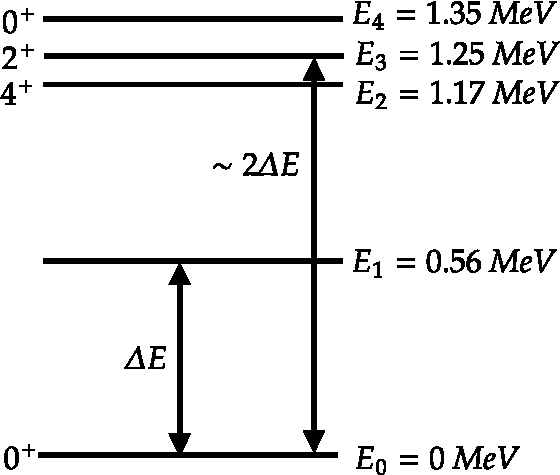
\includegraphics[height=5cm,width=5.5cm]{diagram-20211025-crop}
	\end{figure}
	The spin-parity $j^{p}$ of the level $E_{1}$ is
{	\exyear{NET/JRF(DEC-2018)}}
\begin{tasks}(4)
\task[\textbf{A.}] $1^+$
\task[\textbf{B.}] $1^-$
\task[\textbf{C.}] $2^-$
\task[\textbf{D.}] $2^+$ 
\end{tasks}
\begin{answer}$\left. \right. $\\
Quadrupole oscillations are the lowest order nuclear vibrational mode. The quanta of vibrational energy are called phonons. A quadrupole phonon carries 2 units of angular momentum. Therefore, the parity is $P=(-1)^{2}=+v e$\\
Also, the even-even ground state is $O^{+}$. The 1 phonon excited state is $2^{+}$. The 2 phonons excited states are $0^{+}, 2^{+}, 4^{+}$.\\
\begin{figure}[H]
	\centering
	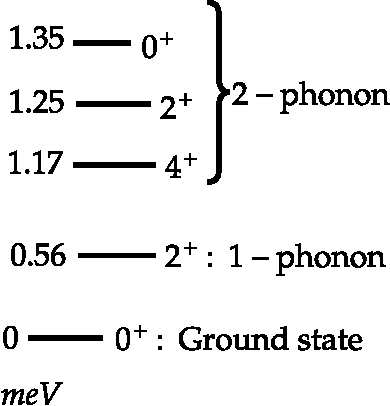
\includegraphics[height=4cm,width=4.5cm]{diagram-20211025(1)-crop}
\end{figure}
So the correct answer is \textbf{Option (D)}
\end{answer}
	\item The Bethe-Weizsacker formula for the binding energy (in MeV) of a nucleus of atomic number $Z$ and mass number $A$ is
	$$
	15.8 A-18.3 A^{2 / 3}-0.714 \frac{Z(Z-1)}{A^{1 / 3}}-23.2 \frac{(A-2 Z)^{2}}{A}
	$$
	The ratio $Z / A$ for the most stable isobar of a $A=64$ nucleus, is nearest to
{	\exyear{NET/JRF(DEC-2019)}}
\begin{tasks}(4)
\task[\textbf{A.}] $0.30$
\task[\textbf{B.}] $0.35$
\task[\textbf{C.}] $0.45$
\task[\textbf{D.}] $0.50$
\end{tasks}
\begin{answer}
\begin{align*}
Z_{0}&=\frac{A}{2+\frac{a_{c}}{2 a_{a}} A^{2 / 3}} \Rightarrow \frac{Z_{0}}{A}=\frac{1}{2+\frac{a_{c}}{2 a_{a}} A^{2 / 3}}\\
\text{given }a_{c}&=0.714\text{ and }a_{a}=23.2\\
\therefore \frac{Z_{0}}{A}&=\frac{1}{2+\frac{0.714}{2 \times 23.2} A^{2 / 3}}=\frac{1}{2+0.015 A^{2 / 3}}\\&=\frac{1}{2+0.015(64)^{2 / 3}}=0.45
\end{align*}
So the correct answer is \textbf{Option (C)}
\end{answer}
	\item A negative muon, which has a mass nearly 200 times that of an electron, replaces an electron in a $L i$ atom. The lowest ionization energy for the muonic $L i$ atom is approximately
{	\exyear{NET/JRF(DEC-2019)}}
\begin{tasks}(2)
\task[\textbf{A.}] The same as that of $\mathrm{He}$
\task[\textbf{B.}] The same as that of normal $L i$
\task[\textbf{C.}]  200 times larger than that of normal $\mathrm{Li}$
\task[\textbf{D.}]  The same as that of normal $\mathrm{Be}$
\end{tasks}
\begin{answer}
\begin{align*}
\intertext{Ionization energy}
I&=\frac{R_{C} R_{\infty}}{n^{2}}(Z-S)^{2}\left(\frac{m^{\prime}}{m_{e}}\right) \Rightarrow I=A\left(\frac{m^{\prime}}{m_{e}}\right)\\
I&=\frac{R_{C} R_{\infty}}{n^{2}}(Z-S)^{2}\left(\frac{m^{\prime}}{m_{e}}\right) \Rightarrow I=A\left(\frac{m^{\prime}}{m_{e}}\right)\\
m^{\prime}&=\frac{7 m_{p} \times m_{e}}{7 m_{p}+m_{e}} \Rightarrow \frac{m^{\prime}}{m_{e}}=\frac{7 \times 1836}{7 \times 1836} \cong 1\\
\therefore I_{L i}&=A
\intertext{For Muonic Li-atom}
m^{\prime}&=\frac{7 m_{p} \times m_{\mu^{-}}}{7 m_{p} \times m_{\mu^{-}}} \cong \frac{7 \times 1836 \times 200 m_{e}^{2}}{(7 \times 1836+200) m_{e}}=197 m_{e}\\
\therefore I_{L i}^{\mu}&=197 A=197 I_{L i}
\intertext{	Thus correct option is (C)}
\intertext{	Note: Answer does not match}
\end{align*}
So the correct answer is \textbf{Option (A)}
\end{answer}
	\item The binding energy $B$ of a nucleus is approximated by the formula $B=a_{1} A-a_{2} A^{2 / 3}-a_{3} Z^{2} A^{-1 / 3}-a_{4}(A-2 Z)^{2} A^{-1}$, where $Z$ is the atomic number and $A$ is the mass number of the nucleus. If $\frac{a_{4}}{a_{2}} \simeq 30$. The atomic number $Z$ for naturally stable isobars (constant value of $A$ ) is
{	\exyear{NET/JRF(JUNE-2020)}}
\begin{tasks}(4)
\task[\textbf{A.}]  $\frac{30 A}{60+A^{2 / 3}}$
\task[\textbf{B.}] $\frac{30 A}{30+A^{2 / 3}}$
\task[\textbf{C.}]  $\frac{60 A}{120+A^{2 / 3}}$
\task[\textbf{D.}] $\frac{120 A}{60+A^{2 / 3}}$
\end{tasks}
\begin{answer}
\begin{align*}
B&=a_{1} A-a_{2} A^{2 / 3}-a_{3} Z^{2} A^{-1 / 3}-a_{4}(A-2 Z)^{2} A^{-1}\\
\text{For most isobar }\frac{\partial B}{\partial Z}&=0 \Rightarrow-\frac{a_{3}(2 Z)}{A^{1 / 3}}-\frac{a_{4} 2(A-2 Z)(-2)}{A}=0\\
\Rightarrow a_{3} \frac{Z}{A^{1 / 3}}&=2 a_{4} \frac{A}{A}-4 a_{4} \frac{Z}{A}\\
\Rightarrow \frac{Z}{A}\left(a_{3} A^{2 / 3}+4 a_{4}\right)&=2 a_{4} \Rightarrow Z=\frac{2 a_{4} A}{a_{3} A^{2 / 3}+4 a_{4}}=\frac{A}{2+\frac{a_{3}}{2 a_{4}} A^{2 / 3}}\\
\Rightarrow Z&=\frac{A}{2+\frac{1}{60} A^{2 / 3}}=\frac{60 A}{120+A^{2 / 3}}
\end{align*}
So the correct answer is \textbf{Option (C)}
\end{answer}
	\item The magnetic moments of a proton and a neutron are $2.792 \mu_{N}$ and $-1.913 \mu_{N}$, where $\mu_{N}$ is the nucleon magnetic moment. The values of the magnetic moments of the mirror nuclei ${ }_{9}^{19} F_{10}$ and ${ }_{10}^{19} \mathrm{Ne}_{9}$, respectively, in the Shell model, are closest to
{	\exyear{NET/JRF(JUNE-2020)}}
\begin{tasks}(2)
\task[\textbf{A.}] $23.652 \mu_{N}$ and $-18.873 \mu_{N}$
\task[\textbf{B.}] $26.283 \mu_{N}$ and $-16.983 \mu_{N}$
\task[\textbf{C.}] $-2.628 \mu_{N}$ and $1.887 \mu_{N}$
\task[\textbf{D.}] $2.628 \mu_{N}$ and $-1.887 \mu_{N}$
\end{tasks}
\begin{answer}
\begin{align*}
{ }_{9}^{19} F_{10}&: p(9): 1 s_{1 / 2}^{2} 1 p_{3 / 2}^{2} 1 p_{1 / 2}^{2} 1 d_{5 / 2}^{2}\\
j&=\frac{5}{2}=2+\frac{1}{2}=l+\frac{1}{2}\\
\left\langle\mu_{Z}\right\rangle_{F^{19}}&=\mu_{N}(i+2.29)=\mu_{N}(2.5+2.29)=4.79 \mu_{N}\\
{ }_{10}^{19} N e_{9}&: N(9): 1 s_{1 / 2}^{2} 1 p_{3 / 2}^{4} 1 p_{1 / 2}^{2} 1 d_{5 / 2}^{1}\\
j&=\frac{5}{2}=l+\frac{1}{2}\\
\left\langle\mu_{z}\right\rangle_{N e^{19}}&=-1.91 \mu_{N}
\intertext{These value are closet to option (D)}
\end{align*}
So the correct answer is \textbf{Option (D)}
\end{answer}
\end{enumerate}
 \colorlet{ocre1}{ocre!70!}
\colorlet{ocrel}{ocre!30!}
\setlength\arrayrulewidth{1pt}
\begin{table}[H]
	\centering
	\arrayrulecolor{ocre}
	\begin{tabular}{|p{1.5cm}|p{1.5cm}||p{1.5cm}|p{1.5cm}|}
		\hline
		\multicolumn{4}{|c|}{\textbf{Answer key}}\\\hline\hline
		\rowcolor{ocrel}Q.No.&Answer&Q.No.&Answer\\\hline
		1&\textbf{C} &2&\textbf{B}\\\hline 
		3&\textbf{C} &4&\textbf{A} \\\hline
		5&\textbf{C} &6&\textbf{D} \\\hline
		7&\textbf{A}&8&\textbf{C}\\\hline
		9&\textbf{A}&10&\textbf{A}\\\hline
		11&\textbf{B} &12&\textbf{C}\\\hline
		13&\textbf{C}&14&\textbf{A}\\\hline
		15&\textbf{C} &16&\textbf{A} \\\hline
		17&\textbf{A}&18&\textbf{B}\\\hline
		19&\textbf{D}&20&\textbf{C}\\\hline
		21&\textbf{A} &22&\textbf{C}\\\hline
		23&\textbf{D} &&\textbf{} \\\hline
		\end{tabular}
\end{table}






\newpage
\begin{abox}
	Practice Set 2 
	\end{abox}
\begin{enumerate}
\item In the nuclear shell model the spin parity of ${ }_{7}^{15} \mathrm{~N}$ is given by
{\exyear{GATE 2010}}
\begin{tasks}(4)
\task[\textbf{A.}] $\frac{1^{-}}{2}$
\task[\textbf{B.}] $\frac{1^{+}}{2}$
\task[\textbf{C.}] $\frac{3^{-}}{2}$
\task[\textbf{D.}] $\frac{3^{+}}{2}$
\end{tasks}
\begin{answer}
\begin{align*}
Z&=7 ;\left(s_{1 / 2}\right)^{2}\left(p_{3 / 2}\right)^{4}\left(p_{1 / 2}\right)^{1} \quad\text{ and }N=8\\
l&=1, J=\frac{1}{2} \Rightarrow\text{ parity }=(-1)^{1}=-1, \\\text{ spin - parity } &=\left(\frac{1}{2}\right)^{-}\\
\text{So the correct answer is} \textbf{ Option (A)}
\end{align*}
\end{answer}
\item The ground state wavefunction of deuteron is in a superposition of $\mathrm{s}$ and $\mathrm{d}$ states. Which of the following is NOT true as a consequence?
{\exyear{GATE 2010}}
\begin{tasks}(1)
\task[\textbf{A.}]  It has a non-zero quadruple moment
\task[\textbf{B.}] The neutron-proton potential is non-central
\task[\textbf{C.}]  The orbital wavefunction is not spherically symmetric
\task[\textbf{D.}]  The Hamiltonian does not conserve the total angular momentum
\end{tasks}
\begin{answer}
So the correct answer is \textbf{Option (D)}
\end{answer}
\item The first three energy levels of ${ }^{228} T h_{90}$ are shown below\\
\begin{figure}[H]
	\centering
	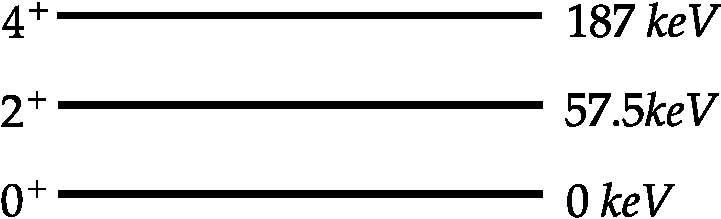
\includegraphics[height=1.5cm,width=6cm]{diagram-20210920-crop}
	\caption{}
	\label{}
\end{figure}
The expected spin-parity and energy of the next level are given by
{\exyear{GATE 2010}}
\begin{tasks}(4)
\task[\textbf{A.}] $\left(6^{+} ; 400 \mathrm{keV}\right)$
\task[\textbf{B.}] $\left(6^{+} ; 300 \mathrm{keV}\right)$
\task[\textbf{C.}] $\left(2^{+} ; 400 \mathrm{keV}\right)$
\task[\textbf{D.}] $\left(4^{+} ; 300 \mathrm{keV}\right)$
\end{tasks}
\begin{answer}
\begin{align*}
\frac{E_{2}}{E_{1}}&=\frac{J_{2}\left(J_{2}+1\right)}{J_{1}\left(J_{1}+1\right)} \Rightarrow \frac{E_{6}}{E_{4}}\\&=\frac{6(6+1)}{4(4+1)} \Rightarrow E_{6}=393 \mathrm{keV}
\end{align*}
So the correct answer is \textbf{Option (A)}
\end{answer}
\item The semi-empirical mass formula for the binding energy of nucleus contains a surface correction term. This term depends on the mass number $A$ of the nucleus as
{\exyear{GATE 2011}}
\begin{tasks}(4)
\task[\textbf{A.}] $A^{-1 / 3}$
\task[\textbf{B.}] $A^{1 / 3}$
\task[\textbf{C.}]  $A^{2 / 3}$
\task[\textbf{D.}] $A$
\end{tasks}
\begin{answer}
So the correct answer is \textbf{Option (C)}
\end{answer}
\item According to the single particles nuclear shell model, the spin-parity of the ground state of ${ }_{8}^{17} O$ is
{\exyear{GATE 2011}}
\begin{tasks}(4)
\task[\textbf{A.}] $\frac{1}{2}$
\task[\textbf{B.}] $\frac{3}{2}$
\task[\textbf{C.}] $\frac{3^{+}}{2}$
\task[\textbf{D.}] $\frac{5^{+}}{2}$
\end{tasks}
\begin{answer}
\begin{align*}
Z&=8\text{ and }N=9 ;\left(s_{1 / 2}\right)^{2}\left(p_{3 / 2}\right)^{4}\left(p_{1 / 2}\right)^{2}\left(d_{5 / 2}\right)^{1}\\
l&=2, J=\frac{5}{2} \Rightarrow\text{ parity }=(-1)^{2}=+1, \\\text{ spin - parity } &=\left(\frac{5}{2}\right)^{+}
\end{align*}
So the correct answer is \textbf{Option (D)}
\end{answer}
\item In the $\beta$ decay process, the transition $2^{+} \rightarrow 3^{+}$, is
{\exyear{GATE 2013}}
\begin{tasks}(1)
\task[\textbf{A.}] Allowed both by Fermi and Gamow-Teller selection rule
\task[\textbf{B.}]  Allowed by Fermi and but not by Gamow-Teller selection rule
\task[\textbf{C.}] Not allowed by Fermi but allowed by Gamow-Teller selection rule
\task[\textbf{D.}] Not allowed both by Fermi and Gamow-Teller selection rule
\end{tasks}
\begin{answer}
\begin{align*}
\intertext{According to Fermi Selection Rule:}
\Delta I&=0, \quad\text{ Parity }=\text{ No Change}
\intertext{According to Gammow-Teller Selection Rule:}
\Delta I&=0, \pm 1, \quad \text{ Parity $=$ No Change}
\intertext{In the $\beta$ decay process, the transition $2^{+} \rightarrow 3^{+}$,}
\Delta I&=\pm 1, \quad\text{ Parity $=$ No Change}
\end{align*}
So the correct answer is \textbf{Option (C)}
\end{answer}
\item Which one of the following is a fermions'?
{\exyear{GATE 2014}}
\begin{tasks}(4)
\task[\textbf{A.}] $\alpha$-particle
\task[\textbf{B.}] ${ }_{4} B e^{7}$ nucleus
\task[\textbf{C.}] Hydrogen atom
\task[\textbf{D.}] Deuteron
\end{tasks}
\begin{answer}
If a nucleus contains odd number of nucleons, it is fermions. If a nucleus contains even number of nucleons, it is a boson.\\\\
So the correct answer is \textbf{Option (B)}
\end{answer}
\item The atomic masses of ${ }_{63}^{152} E u,{ }_{62}^{152} \mathrm{Sm},{ }_{1}^{1} H$ and neutron are $151.921749,151.919756$, $1.007825$ and $1.008665$ in atomic mass units (amu), respectively. Using the above information, the $Q$ - value of the reaction ${ }_{63}^{152} E u+n \rightarrow_{62}^{152} S m+p$ is--------------- $\times 10^{-3}$ amu (upto three decimal places)
{\exyear{GATE 2015}}
\begin{answer}
\begin{align*}
Q&=152.930414-(152.927581)=2.833 \times 10^{-3} a.m.u.
\end{align*}
So the correct answer is $2.833$
\end{answer}
\item In the nuclear shell model, the potential is modeled as $V(r)=\frac{1}{2} m \omega^{2} r^{2}-\lambda \vec{L} \cdot \vec{S}, \lambda>0$. The correct spin-parity and isospin assignments for the ground state of ${ }_{6}^{13} C$ is
{\exyear{GATE 2015}}
\begin{tasks}(4)
\task[\textbf{A.}] $\frac{1^{-}}{2} ; \frac{-1}{2}$
\task[\textbf{B.}] $\frac{1^{+}}{2} ; \frac{-1}{2}$
\task[\textbf{C.}] $\frac{3^{+}}{2} ; \frac{1}{2}$
\task[\textbf{D.}] $\frac{3^{-}}{2} ; \frac{-1}{2}$
\end{tasks}
\begin{answer}
\begin{align*}
{ }^{13} C_{6}, \quad N&=7, Z=6,\text{ for }N\\&=7 ;\left(1 S_{\frac{1}{2}}\right)^{2}\left(1 P_{\frac{3}{2}}\right)^{4}\left(P_{\frac{1}{2}}\right)^{1} \Rightarrow j=\frac{1}{2} \text{and }l=1\\
\text{	Thus spin- parity is }&\left(\frac{1}{2}\right)^{-}.
\end{align*}
So the correct answer is \textbf{Option (A)}
\end{answer}
\item According to the nuclear shell model, the respective ground state spin-parity values of ${ }_{8}^{15} O$ and ${ }_{8}^{17} O$ nuclei are
{\exyear{GATE 2016}}
\begin{tasks}(4)
\task[\textbf{A.}] $\frac{1^{+}}{2}, \frac{1^{-}}{2}$
\task[\textbf{B.}] $\frac{1}{2}^{-}, \frac{5^{+}}{2}$
\task[\textbf{C.}] $\frac{3^{-}}{2}, \frac{5^{+}}{2}$
\task[\textbf{D.}] $\frac{3^{-}}{2}, \frac{1^{-}}{2}$
\end{tasks}
\begin{answer}
\begin{align*}
{ }_{8}^{15} O ; Z&=8\text{ and }N=7 ; \\ N&=7:\left(s_{1 / 2}\right)^{2}\left(p_{3 / 2}\right)^{4}\left(p_{1 / 2}\right)^{1}\\
\Rightarrow j&=\frac{1}{2}\text{ and }l=1 .\text{ Thus spin and parity} =\left(\frac{1}{2}\right)^{-}\\
{ }_{8}^{17} O ; Z&=8\text{ and }N=9 ; \\ N&=9:\left(s_{1 / 2}\right)^{2}\left(p_{3 / 2}\right)^{4}\left(p_{1 / 2}\right)^{2}\left(d_{5 / 2}\right)^{1}\\
\Rightarrow j&=\frac{5}{2}\text{ and }l=2.\text{ Thus spin and parity} =\left(\frac{5}{2}\right)^{+}
\end{align*}
So the correct answer is \textbf{Option (B)}
\end{answer}
\item The $\pi^{+}$decays at rest to $\mu^{+}$and $v_{\mu}$. Assuming the neutrino to be massless, the momentum of the neutrino is.................. $\mathrm{MeV} / \mathrm{c}$. (up to two decimal places)\\ $\left(m_{\pi}=139 \mathrm{MeV} / \mathrm{c}^{2}, m_{\mu}=105 \mathrm{MeV} / \mathrm{c}^{2}\right)$
{\exyear{GATE 2017}}
\begin{answer}
\begin{align*}
E_{v}&=\frac{\left(m_{\pi}^{2}-m_{\mu}^{2}\right) c^{2}}{2 m_{\pi}}=p \times c\\
\text{	So }p&=\frac{\left(m_{\pi}^{2}-m_{\mu}^{2}\right) c}{2 m_{\pi}}\\&=\frac{19321-11025}{2 \times 139 c}=\frac{29.84}{c}(\mathrm{MeV})
\end{align*}
So the correct answer is $29.84$
\end{answer}
\item For nucleus ${ }^{164} \mathrm{Er}$, a $J^{\pi}=2^{+}$state is at $90 \mathrm{keV}$. Assuming ${ }^{164} \mathrm{Er}$ to be a rigid rotor, the energy of its $4^{+}$state is -------------$\mathrm{keV}$ (up to one decimal place)
{\exyear{GATE 2018}}
\begin{answer}$\left. \right. $
\begin{figure}[H]
	\centering
	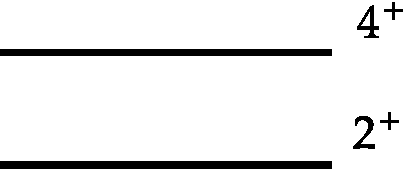
\includegraphics[height=1.5cm,width=3.5cm]{diagram-20210920(3)-crop}
\end{figure}
\begin{align*}
E_{J}&=h c B J(J+1)\\
E_{2^{+}}&=h c B 2(2+1)\text{ and }E_{4^{+}}=h c B 4(4+1)\\
\text{Then, }\frac{E_{4^{+}}}{E_{2^{+}}}&=\frac{20}{6} \Rightarrow E_{4^{+}}\\&=\frac{20}{6} \times 90 \mathrm{keV}=300 \mathrm{keV}
\end{align*}
\end{answer}
\end{enumerate}
 \colorlet{ocre1}{ocre!70!}
\colorlet{ocrel}{ocre!30!}
\setlength\arrayrulewidth{1pt}
\begin{table}[H]
	\centering
	\arrayrulecolor{ocre}
	\begin{tabular}{|p{1.5cm}|p{1.5cm}||p{1.5cm}|p{1.5cm}|}
		\hline
		\multicolumn{4}{|c|}{\textbf{Answer key}}\\\hline\hline
		\rowcolor{ocrel}Q.No.&Answer&Q.No.&Answer\\\hline
		1&\textbf{B} &2&\textbf{D}\\\hline 
		3&\textbf{A} &4&\textbf{C} \\\hline
		5&\textbf{D} &6&\textbf{C} \\\hline
		7&\textbf{B}&8&\textbf{2.833}\\\hline
		9&\textbf{A}&10&\textbf{B}\\\hline
		11&\textbf{29.84} &12&\textbf{300}\\\hline
		
	\end{tabular}
\end{table}


\newpage
\begin{abox}
	Practice Set 3 
\end{abox}
\begin{enumerate}
	\item Two spherical nuclei have mass numbers 216 and 64 with their radii $R_{1}$ and $R_{2}$, respectively. The ratio $\frac{R_{1}}{R_{2}}$ is
{	\exyear{IIT JAM 2009}}
\begin{tasks}(4)
\task[\textbf{A.}]1
\task[\textbf{B.}]1.5
\task[\textbf{C.}]2
\task[\textbf{D.}]2.5
\end{tasks}
\item The variation of binding energy per nucleon with respect to the mass number of nuclei is shown in the figure.
Consider the following reactions:
(i) ${ }_{92}^{238} U \rightarrow_{82}^{206} P b+10 P+22 n$
(ii) ${ }_{92}^{238} \mathrm{U} \rightarrow{ }_{82}^{206} \mathrm{~Pb}+8{ }_{2}^{4} \mathrm{He}+6 e^{-}$
Which one of the following statements is true for the given decay modes of ${ }_{92}^{238} U$ ?
{\exyear{IIT JAM 2015}}
\begin{figure}[H]
	\centering
	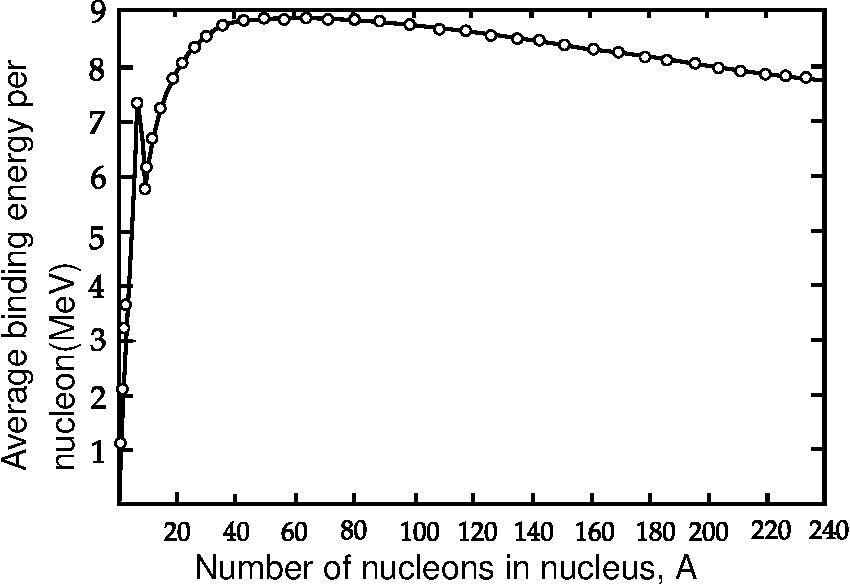
\includegraphics[height=5cm,width=8cm]{diagram-20211122(45)-crop}
\end{figure}
\begin{tasks}(2)
	\task[\textbf{A.}]Both (i) and (ii) are allowed
	\task[\textbf{B.}]Both (i) and (ii) are forbidden
	\task[\textbf{C.}](i) is forbidden and (ii) is allowed
	\task[\textbf{D.}](i) is allowed and (ii) is forbidden
\end{tasks}
	\item For an atomic nucleus with atomic number $Z$ and mass number $A$, which of the following is (are) correct?
{	\exyear{IIT JAM 2017}}
\begin{tasks}(1)
\task[\textbf{A.}](a) Nuclear matter and nuclear charge are distributed identically in the nuclear volume
\task[\textbf{B.}]Nuclei with $Z>83$ and $A>209$ emit $\alpha$ - radiation
\task[\textbf{C.}] The surface contribution to the binding energy is proportional to $A^{2 / 3}$
\task[\textbf{D.}]$\beta$ - decay occurs when the proton to neutron ratio is large, but not when it is small
\end{tasks}
	\item The relation between the nuclear radius $(R)$ and the mass number $(A)$, given by $R=1.2 A^{1 / 3} \mathrm{fm}$, implies that
{	\exyear{IIT JAM 2019}}
\begin{tasks}(1)
\task[\textbf{A.}]The central density of nuclei is independent of $A$
\task[\textbf{B.}]The volume energy per nucleon is a constant
\task[\textbf{C.}]The attractive part of the nuclear force has a long range
\task[\textbf{D.}]The nuclear force is charge dependent
\end{tasks}
		\item A duetron strikes ${ }_{8} \mathrm{O}^{16}$ nucleus with subsequent emission of alpha particle. Identify the nucleus so produced
	\begin{tasks}(2)
		\task[\textbf{A.}] ${ }_{3} \mathrm{Li}^{7}$
		\task[\textbf{B.}]  ${ }_{5} \mathrm{~B}^{10}$
		\task[\textbf{C.}]${ }_{7} \mathrm{~N}^{13}$
		\task[\textbf{D.}]${ }_{7} \mathrm{~N}^{14}$
	\end{tasks}
		\item For a nuclear fusion process, suitable nuclei are
	\begin{tasks}(2)
		\task[\textbf{A.}]any Nuclei 
		\task[\textbf{B.}] heavy Nuclei
		\task[\textbf{C.}]light Nuclei
		\task[\textbf{D.}]nuclei lying in the middle of periodic table
	\end{tasks}
		\item A nuclear reaction is given by $\mathrm{Z}^{\mathrm{X}}{\mathrm{A}} \rightarrow \mathrm{Z}_{+1} \mathrm{Y}^{\mathrm{A}}+{ }_{-1} \mathrm{e}^{0}+\bar{v}$, represents
	\begin{tasks}(2)
		\task[\textbf{A.}] fission
		\task[\textbf{B.}] $\beta$-decay
		\task[\textbf{C.}]$\sigma$-decay
		\task[\textbf{D.}]fusion
	\end{tasks}
	\item A nucleus ${ }_{n}^{m} X$ emits one $\alpha$-particle and two $\beta$-particles. The resulting nucleus is
\begin{tasks}(1)
	\task[\textbf{A.}] $\underset{\mathrm{n}-4}{\mathrm{~m}-6} \mathrm{Z}$
	\task[\textbf{B.}] $\underset{\mathrm{n}}{\mathrm{m}-6} \mathrm{Z}$
	\task[\textbf{C.}]${ }_{\mathrm{n}}^{\mathrm{m}-4} \mathrm{X}$
	\task[\textbf{D.}]${ }_{\mathrm{n}-2}^{\mathrm{m}-4} \mathrm{Y}$
\end{tasks}
	\item The mass of a ${ }_{3}^{7} L i$ nucleus is $0.042 \mathrm{u}$ less than the sum of the masses of all its nucleons. The binding energy per nucleon of ${ }_{3}^{7} L i$ nucleus is nearly
\begin{tasks}(2)
	\task[\textbf{A.}]$46 \mathrm{MeV}$
	\task[\textbf{B.}] $5.6 \mathrm{MeV}$
	\task[\textbf{C.}]$3.9 \mathrm{MeV}$
	\task[\textbf{D.}]$23 \mathrm{MeV}$ 
\end{tasks}		
	\item A nucleus disintegrated into two nuclear parts which have their velocities in the ratio of $2: 1$. The ratio of their nuclear sizes will be
\begin{tasks}(2)
	\task[\textbf{A.}]  $3^{1 / 2}: 1$
	\task[\textbf{B.}]  $1: 2^{1 / 3}$
	\task[\textbf{C.}]$2^{1 / 3}: 1$
	\task[\textbf{D.}]$1: 3^{1 / 2}$
\end{tasks}	
	
	
	
	
	
\end{enumerate}